\begin{figure}[H]
\centering
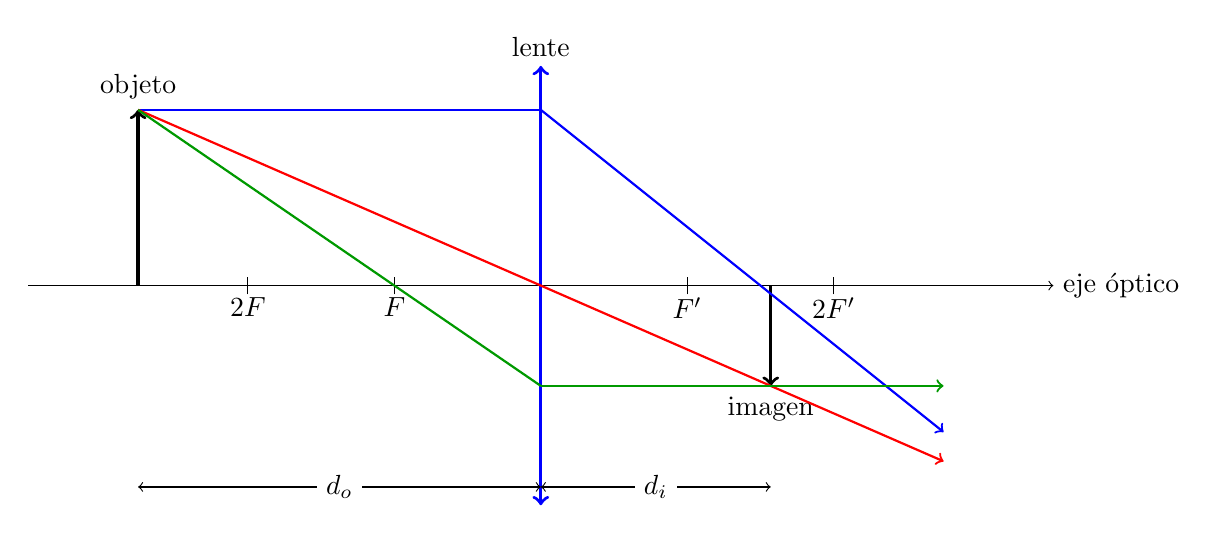
\begin{tikzpicture}[scale=0.93]
  \draw[->] (-7,0) -- (7,0) node[right] {eje óptico};
  \draw[<->,very thick,blue] (0,-3) -- (0,3);
  \node[above] at (0,3) {lente};
  \foreach \x/\lab in {-4/{2F},-2/F,2/{F'},4/{2F'}}{
    \draw (\x,-0.12) -- (\x,0.12) node[below=4pt] {$\lab$};
  }
  \draw[->,very thick] (-5.5,0) -- (-5.5,2.4) node[above] {objeto};
  \draw[->,very thick] (3.14,0) -- (3.14,-1.37) node[below] {imagen};
  \draw[blue,thick] (-5.5,2.4) -- (0,2.4);
  \draw[->,blue,thick] (0,2.4) -- (5.5,-2.0);
  \draw[red,thick,->] (-5.5,2.4) -- (5.5,-2.4);
  \draw[green!60!black,thick] (-5.5,2.4) -- (-2,0) -- (0,-1.37);
  \draw[->,green!60!black,thick] (0,-1.37) -- (5.5,-1.37);
  \draw[<->] (-5.5,-2.75) -- (0,-2.75) node[midway,fill=white] {$d_o$};
  \draw[<->] (0,-2.75) -- (3.14,-2.75) node[midway,fill=white] {$d_i$};
\end{tikzpicture}
\caption{Construcción de una imagen real mediante los tres rayos principales de una lente convergente.}
\end{figure}